\documentclass[main.tex]{subfile}

\begin{document}

\section{Sine Wave Decomposition} 
\label{sec:sections}

To show the affects of the Fourier series on the square wave we first present an
$8^{th}$ order Butterworth filter with a cut-off frequency at $4f$. Where $f$
is the frequency of the square wave. Note how, although their is a phase shift
of the output of the filter, the general shape of the square wave is maintained.
With a higher order filter an even more apparent square wave form will exist.

\begin{figure}[H]
    \begin{center}
      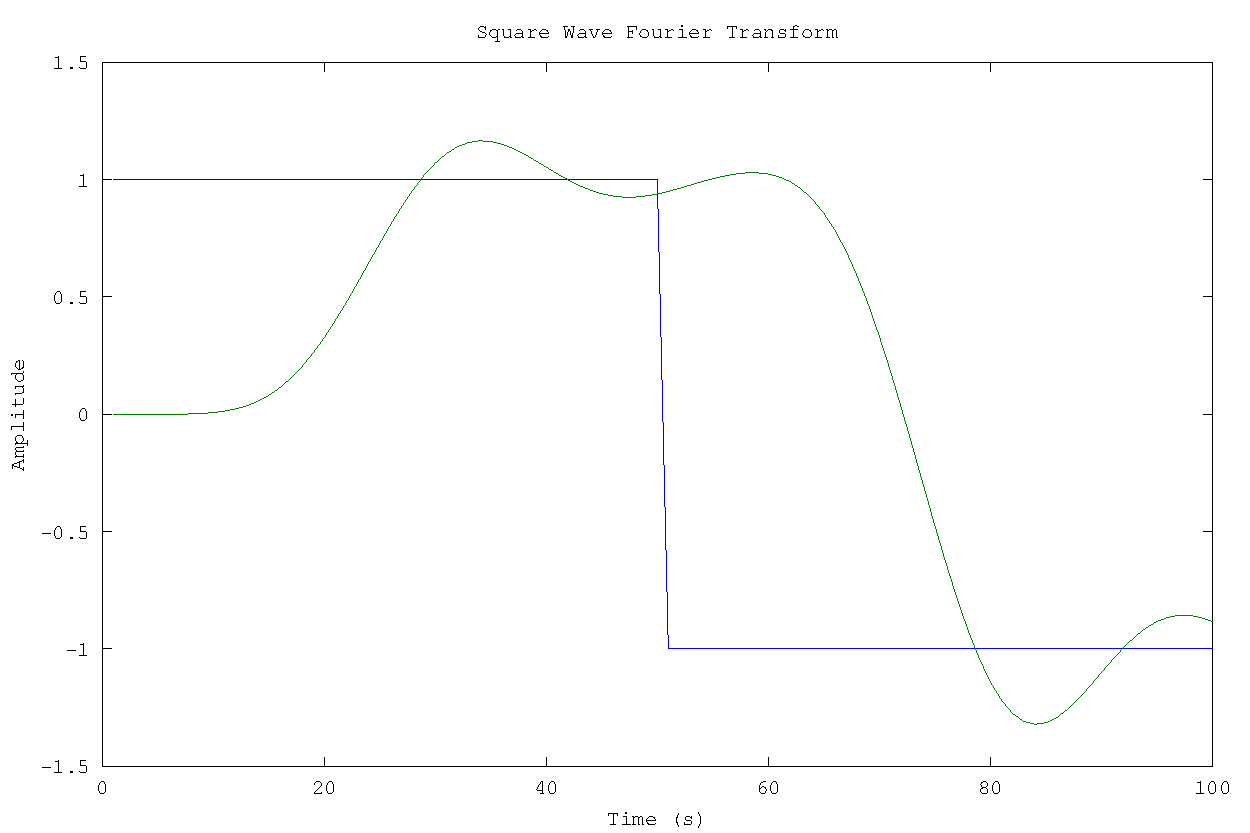
\includegraphics[width=\linewidth]{sqrWave.pdf}
    \end{center}
    \caption{sqrPlot}
    \label{fig:sqrPlot}
  \end{figure}

As a final exercise we wish to show how the number of terms in the Fourier series
expansion relate to the approximation of a square wave. \figref{sinPlot} show
the plot of the terms found in \tabref{termExpansion}. Note how as the number of
terms increases the more the sine wave approximates the square wave. This is due
to a wider band of frequencies used to represent the square wave. As the
summation in \eqref{fSqrWave} approaches an infinite amount of terms the widest
frequency band is covered and (theoretically) a perfect representation of a
square wave is given. Practically however, at least $3 - 10$ terms is enough to
represent most simple signals - indeed, in some cases only $2$ terms are used
such as linearizing pendulum models.
 
\begin{figure}[H]
	\begin{center}
		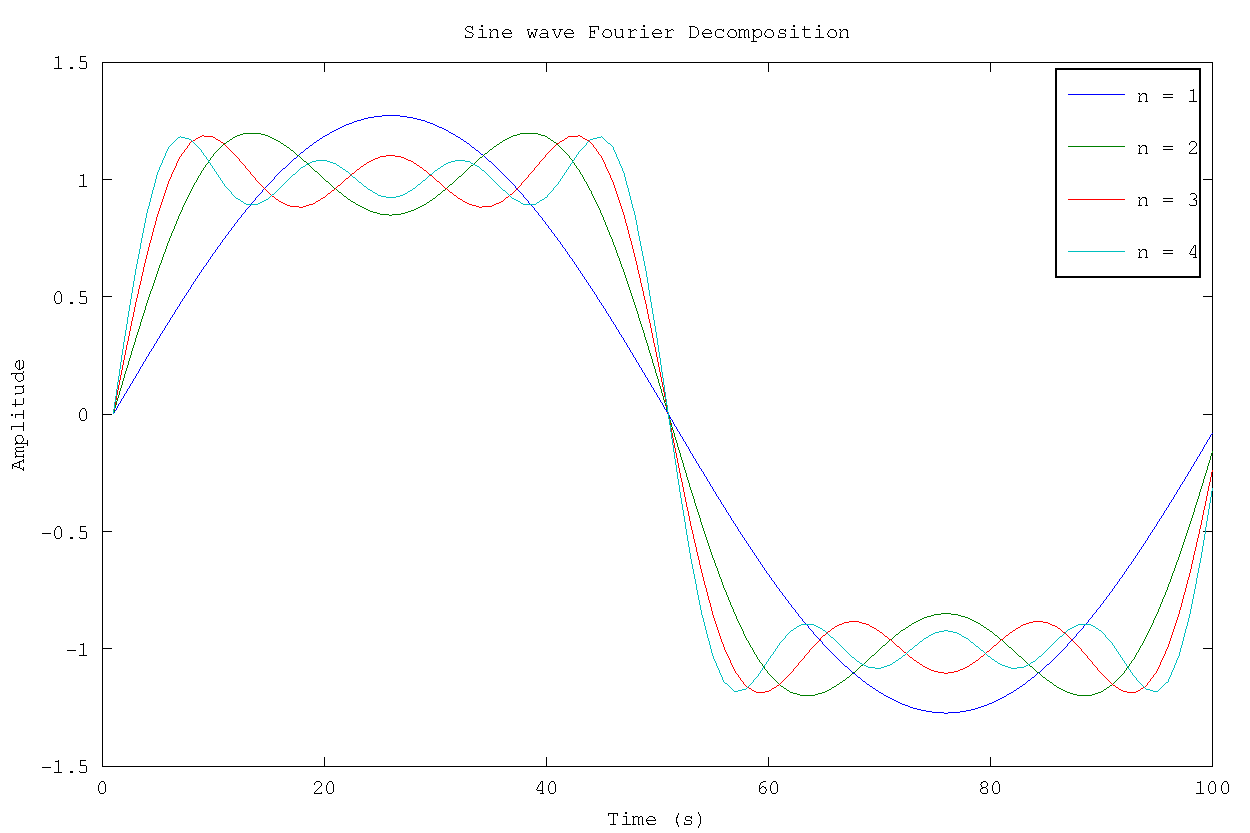
\includegraphics[width=\linewidth]{sinWaves.pdf}
	\end{center}
	\caption{Sine Wave Decomposition}
	\label{fig:sinPlot}
\end{figure}

% section sections (end)

\end{document}
